\section{Design Specification}
\subsection{Project Description}
The scenario for this project describes a city in need of a traffic light control system for their busy intersection.
This project provides a system that satisfies the requirements for the intersection. The road running from North to South is a busy four-lane street with turn lanes,
while the road running from East to West is a small two-lane country road. To allow for optimal traffic flow through the intersection,
the traffic on the busy road is given priority unless there are cars waiting for a certain period of time on the small road or in the turn lanes.

\subsection{Constraints}
\emph{The timing for the controller is as follows:}\\[5mm]
The N-S signal is green by default.\\[5mm]
If there are cars waiting in the N-S turn lane for longer than 15 seconds, the N-S signal will cycle green~$\rightarrow$~yellow~$\rightarrow$~red, followed by the green arrow for 15 seconds.
The N-S signal finally cycles green~arrow~$\rightarrow$~yellow arrow~$\rightarrow$~green, and will stay green for at least 30 seconds.\\[5mm]
If there are cars waiting in the E-W turn lane for longer than 15 seconds, the N-S signal will cycle green~$\rightarrow$~yellow~$\rightarrow$~red, followed by the E-W green light for 15 seconds.
The E-W signal will then cycle green~$\rightarrow$~yellow~$\rightarrow$~red, after which the N-S signal turns green and will stay green for at least 30 seconds.

\section{Logic Design}
\subsection{Details}
\subsection{Diagram}
\includegraphics[scale=0.50]{LogicDiagram.png}

\section{Circuitry}
\subsection{Bill of Materials}
\begin{table}[h]
\begin{tabular}{|r|c|c|}
\hline
\multicolumn{1}{|c|}{\textit{Item}} & \textit{Quantity} & \textit{Unit} \\ \hline
LED, Red & 4 & EA \\ \hline
LED, Green & 6 & EA \\ \hline
LED, Yellow & 6 & EA \\ \hline
Resistor, 1K$\,\mathrm\Omega$ & 4 & EA \\ \hline
Resistor, 330$\,\mathrm\Omega$ & 4 & EA \\ \hline
Induction Proximity Sensor & 4 & EA \\ \hline
Xilinx XC2C256 Development Board & 1 & EA \\ \hline
Arduino Uno Board & 1 & EA \\ \hline
\end{tabular}
\end{table}

\subsection{Circuit Diagram}
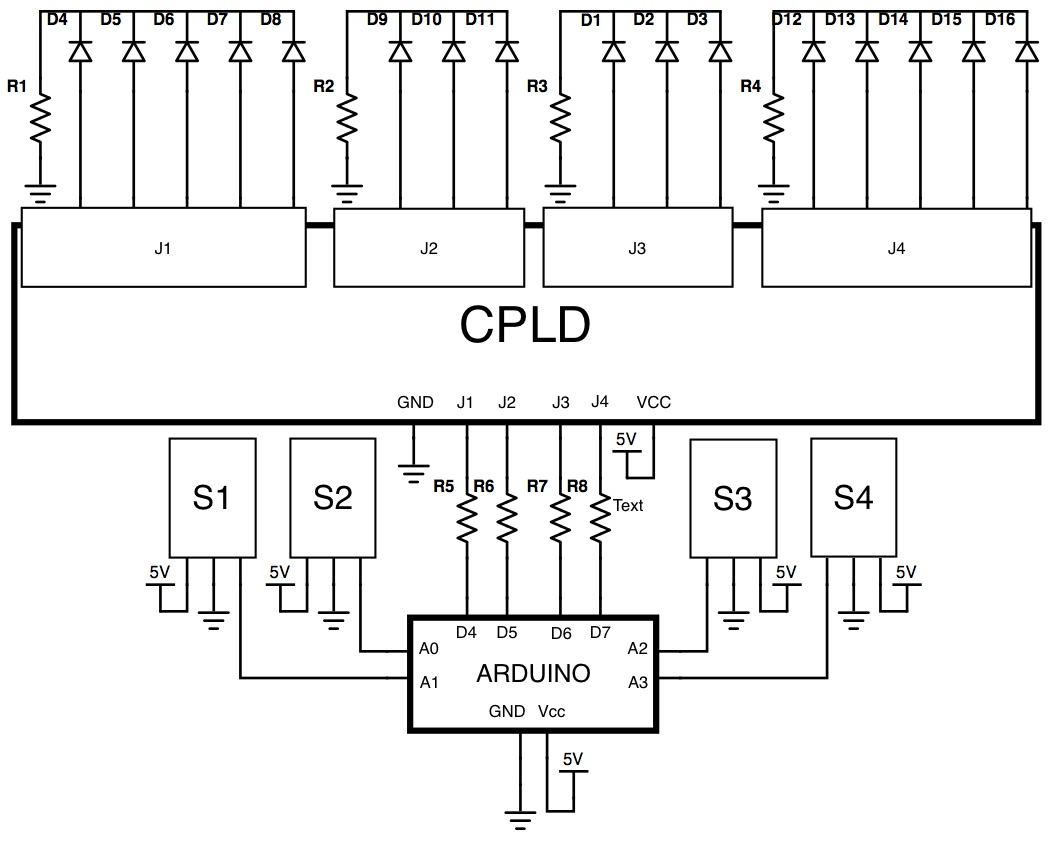
\includegraphics[scale=0.50]{0623151841.jpg}

\section{Prototype Construction and Testing}
\subsection{Testing Process}
Before we could begin testing, several things had to be put in place. Before we could connect anything, the CPLD had to be programmed.
Next, the stoplight assemblies had to be built and connected to the correct pins on the CPLD.
Then we needed to have the Arduino programmed, and wired to both the sensors and the CPLD.
Finally, after everything was properly connected, we had to provide the electronics with power.
Once we had everything connected and powered, we could start testing the assembly. During the testing process, the Arduino was programmed to
transmit data from the sensors via the serial port so we could monitor the sensor readings in real time.
This allowed us to fine-tune the triggering thresholds and correct any problems with the Arduino as we found them.
We powered up the system and used bits of metal to trigger the sensors. Then we simply watched the stoplights run through the cycles. If we noticed
some discrepancy with the lights, be it an error in the cycle, or a defective LED, we took the appropriate steps to resolve the problem,
continuing until there were no further errors.
\subsection{Workflow Diagram}
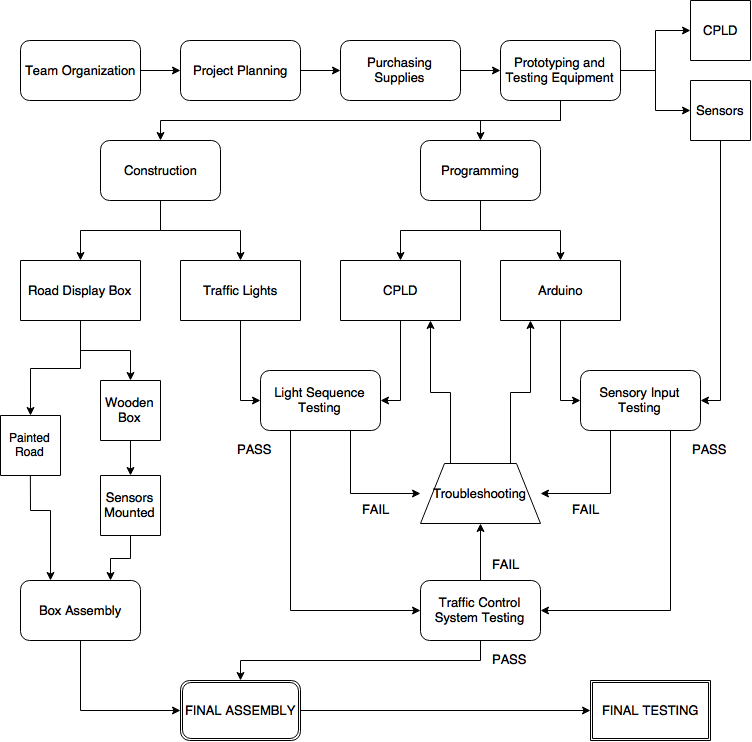
\includegraphics[scale=0.75]{DIGITALFLOW.png}